\documentclass[11pt]{article}
\usepackage[utf8]{inputenc}
\usepackage[margin=1in]{geometry}
\usepackage{amsmath,amssymb}
\usepackage{booktabs}
\usepackage{hyperref}
\usepackage{setspace}
\usepackage{float}
\usepackage{enumitem}
\usepackage{graphicx}
\usepackage{xcolor}
\onehalfspacing

\hypersetup{colorlinks=true,linkcolor=blue!70!black,citecolor=blue!70!black,urlcolor=blue!70!black}

\title{\textbf{Volatility-Managed Factor Portfolios:\\A Replication and Extension on the\\Fama-French Five Factors and Momentum}}
\author{Tanishk Yadav\\[2pt]\textit{MS Financial Engineering}\\New York University, Tandon School of Engineering\\New York, NY, USA}
\date{}

\begin{document}
\maketitle

\begin{abstract}
\noindent
We replicate and extend Moreira and Muir (2017) by volatility-managing the Fama-French five factors plus the momentum factor over 1963 to 2026, using daily data from the Kenneth French Data Library. Each factor's exposure is scaled by the inverse of its prior-month realized variance, so the leverage decision uses only past information. Regressing the managed factor on the original (the Moreira-Muir spanning test, with Newey-West standard errors) gives an honest, factor-dependent answer: volatility timing earns large and statistically significant alpha on the crash-prone factors, momentum (8.9\% per year, $t=5.0$) and profitability (RMW, 2.3\% per year, $t=2.9$), while it adds nothing for size, value, or investment, and the market factor's managed alpha is positive but insignificant over the full sample. Volatility-managed momentum raises the annualized Sharpe ratio from 0.51 to 0.89 (0.81 net of a 14 basis point per turn transaction cost). The results are consistent with Barroso and Santa-Clara (2015): the factors that benefit are those whose left-tail crashes cluster in high-volatility states. We treat the study as performance attribution rather than a live strategy, reporting turnover and net-of-cost Sharpe throughout, and we include sector-level factor attribution and a sector-momentum baseline as context.

\medskip
\noindent\textbf{Keywords:} volatility-managed portfolios, factor timing, Moreira-Muir, momentum, Fama-French, Newey-West
\end{abstract}

\section{Introduction}

A long literature treats factor premia as compensation for risk that is, on average, constant through time. Moreira and Muir (2017) challenge the practical implication of that view: because realized volatility is persistent and only weakly related to next-period expected returns, an investor can scale exposure down when volatility is high and up when it is low, and earn a higher Sharpe ratio than buy-and-hold. This paper reproduces that result on the Fama-French five factors and momentum, asks which factors actually benefit, and is careful to separate a real timing signal from data-snooping.

The contribution is threefold. First, a clean, no-lookahead implementation of the volatility-managed construction on six factors over six decades. Second, an honest cross-factor verdict: the gains are concentrated, not universal. Third, two secondary analyses (sector factor attribution and a sector-momentum baseline) that motivate why timing a factor by its own variance is more tractable than naive cross-sectional momentum.

\section{Methodology}

\subsection{Data}

The volatility-managed study uses daily factor returns from the Kenneth French Data Library: the five Fama-French factors (Mkt-RF, SMB, HML, RMW, CMA) and the momentum factor (Mom), from July 1963 through April 2026. The secondary attribution analysis additionally uses the eleven Sector SPDR ETFs (XLK, XLF, XLV, XLY, XLP, XLE, XLI, XLB, XLU, XLRE, XLC), 2015 to 2025. No API keys are required.

\subsection{Volatility-Managed Construction}

For a factor with monthly return $f_m$, the volatility-managed version is
\begin{equation}
    f^{\sigma}_m = \frac{c}{\mathrm{RV}_{m-1}}\, f_m,
\end{equation}
where $\mathrm{RV}_{m-1}$ is the realized variance of the factor over the prior month, computed as the sum of squared daily returns within that month, and $c$ is a single constant chosen so that $f^{\sigma}$ matches the full-sample volatility of $f$. The timing signal $1/\mathrm{RV}_{m-1}$ depends only on past data, so the leverage choice is genuinely out of sample; $c$ is a scale-only normalization that affects neither the Sharpe ratio nor the spanning-regression $t$-statistic, and exists purely so the two series are comparable.

\subsection{Spanning Test}

The central test regresses the managed factor on the original:
\begin{equation}
    f^{\sigma}_m = \alpha + \beta\, f_m + \varepsilon_m .
\end{equation}
A positive and significant $\alpha$ means the managed factor delivers return that a static position in the original factor cannot span. Because the residuals are serially correlated and heteroskedastic, $t$-statistics use Newey-West (HAC) standard errors with six lags. We annualize $\alpha$ by multiplying the monthly estimate by twelve.

\subsection{Transaction Costs}

The $1/\mathrm{RV}$ weights imply time-varying leverage, so we charge 14 basis points per unit of month-over-month change in the (scaled) weight, in the spirit of the cost robustness checks in Moreira and Muir (2017), and report the resulting net Sharpe ratio alongside average turnover.

\section{Results: Volatility-Managed Factors}

Table \ref{tab:vm} reports the original and managed Sharpe ratios (gross and net of costs), the spanning alpha, its Newey-West $t$-statistic, and average turnover for each of the six factors over the full sample.

\begin{table}[H]
    \centering
    \begin{tabular}{lcccccc}
        \toprule
        \textbf{Factor} & \textbf{Sharpe} & \textbf{Sharpe} & \textbf{Sharpe} & \textbf{Alpha} & \textbf{$t$} & \textbf{Turnover} \\
         & (orig.) & (managed) & (net) & (ann.) & (NW) & \\
        \midrule
        Momentum (Mom)        & 0.51 & \textbf{0.89} & 0.81 & \textbf{+8.9\%} & \textbf{5.03} & 0.75 \\
        Profitability (RMW)   & 0.41 & \textbf{0.54} & 0.41 & \textbf{+2.3\%} & \textbf{2.87} & 0.59 \\
        Market (Mkt-RF)       & 0.48 & 0.46 & 0.40 & +2.1\% & 1.37 & 0.60 \\
        Value (HML)           & 0.37 & 0.35 & 0.26 & +1.4\% & 1.21 & 0.56 \\
        Investment (CMA)      & 0.42 & 0.32 & 0.19 & +0.3\% & 0.45 & 0.54 \\
        Size (SMB)            & 0.15 & 0.09 & 0.01 & $-0.2$\% & $-0.18$ & 0.47 \\
        \bottomrule
    \end{tabular}
    \caption{Volatility-managed factors, monthly, 1963 to 2026. Alpha is the annualized intercept from the spanning regression $f^{\sigma}=\alpha+\beta f+\varepsilon$ with Newey-West (6-lag) $t$-statistics. Net Sharpe charges 14 bps per unit of leverage turnover.}
    \label{tab:vm}
\end{table}

The verdict is factor-dependent. Volatility timing is strongly profitable for \textbf{momentum} (alpha 8.9\% per year, $t=5.0$; the managed Sharpe of 0.89 survives costs at 0.81) and significantly profitable for \textbf{profitability} ($t=2.9$). Both are factors with pronounced negative volatility-return dynamics and fat left tails, exactly where Barroso and Santa-Clara (2015) show that momentum's worst crashes cluster in high-volatility states; scaling down into those states sidesteps the crashes. By contrast, timing \textbf{size}, \textbf{value}, and \textbf{investment} adds turnover without alpha, and the \textbf{market} factor's managed alpha, while positive, is insignificant over the full 1963 to 2026 window, weaker than in Moreira and Muir's original sample and consistent with partial decay after publication.

\begin{figure}[H]
    \centering
    
\includegraphics[width=\textwidth]{images/cum_mkt.png}
    \caption{Cumulative excess return of the volatility-managed market factor versus buy-and-hold.}
    \label{fig:cum_mkt}
\end{figure}

\begin{figure}[H]
    \centering
    
\includegraphics[width=0.9\textwidth]{images/sharpe_bars.png}
    \caption{Annualized Sharpe ratio, original versus volatility-managed, across the six factors. The gains are concentrated in momentum and profitability.}
    \label{fig:sharpe_bars}
\end{figure}

We stress that this is performance attribution, not a deployable strategy: the inverse-variance weights can imply large leverage, so a real implementation would cap leverage, which would shrink the gains. The turnover and net-of-cost columns make the implementation drag explicit.

\section{Secondary Analyses}

\subsection{Sector Factor Attribution}

Estimating Fama-French three-factor, Carhart four-factor, and five-factor models by OLS on the eleven sector ETFs confirms expected structure: the models explain 92 to 93\% of the technology sector's (XLK) daily return variance, with a market beta above 1.0, a negative SMB loading (large-cap bias), and a negative HML loading (growth tilt); adding momentum and profitability improves fit. Rolling 252-day regressions (Figure \ref{fig:rolling_betas}) show that these exposures are non-stationary, with a market-wide correlation spike in the 2020 crash and the 2022 rotation from growth to value.

\begin{figure}[H]
    \centering
    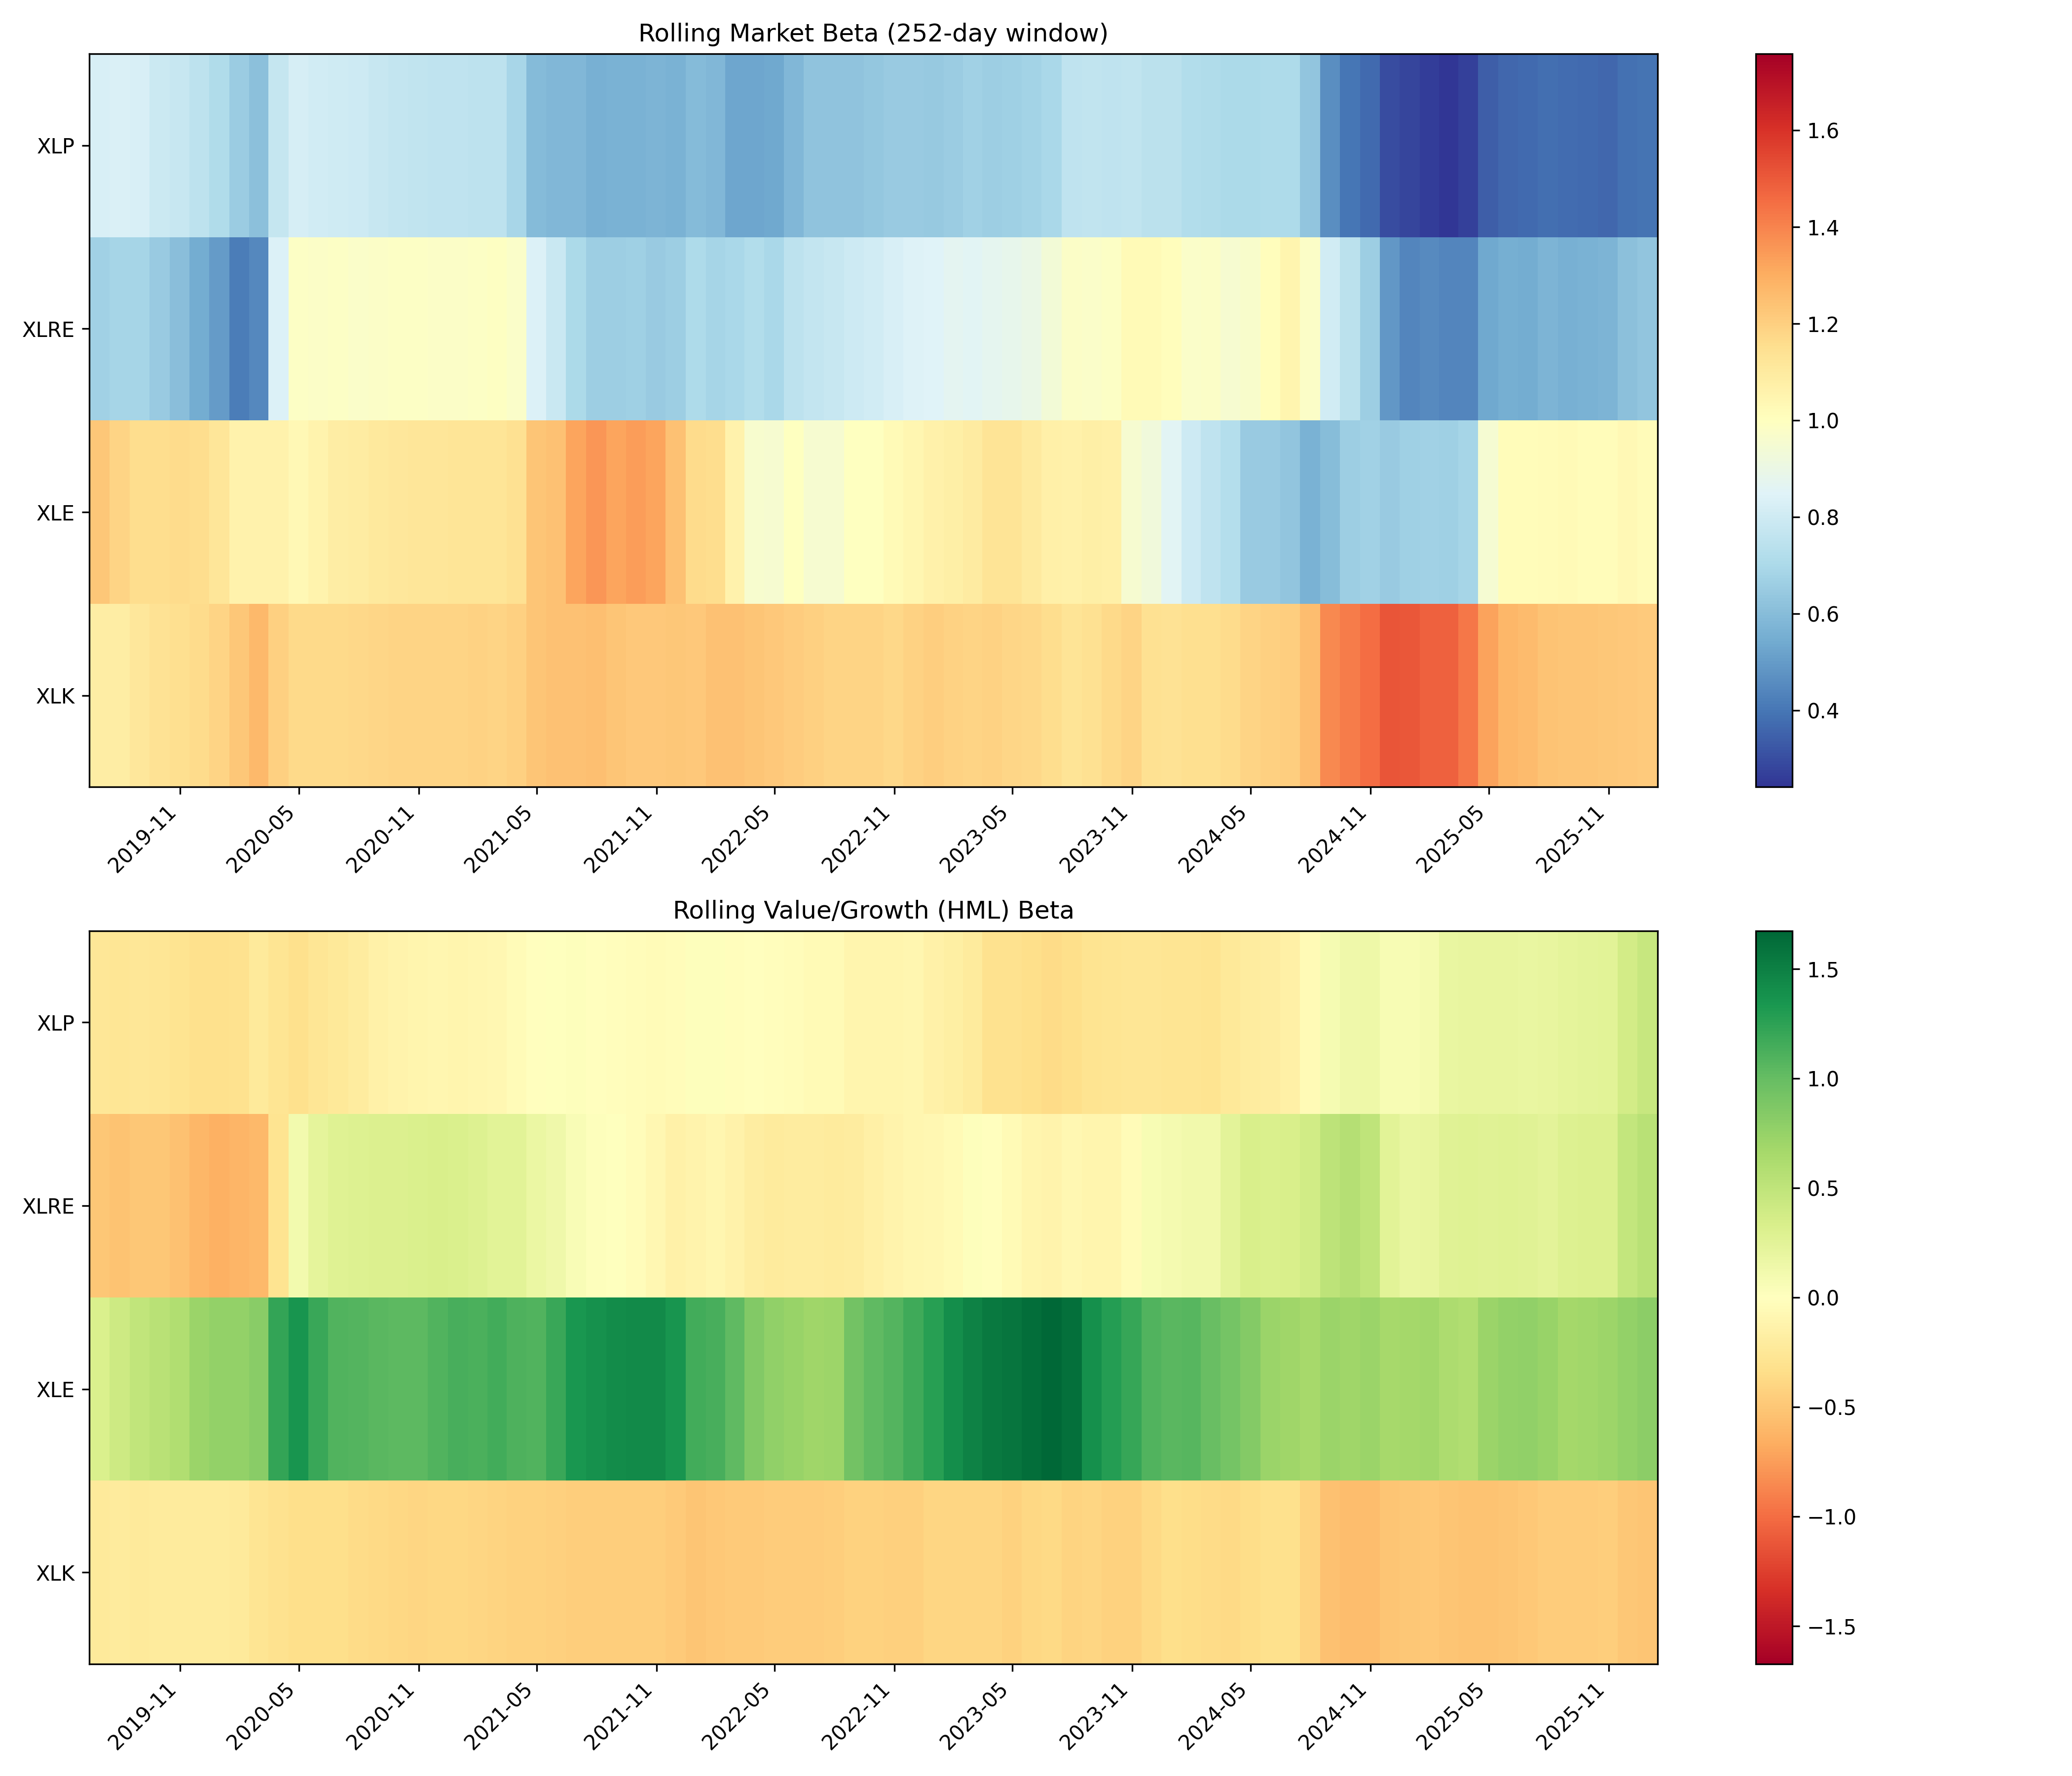
\includegraphics[width=\textwidth]{images/rolling_betas.png}
    \caption{Rolling 252-day market and HML betas for selected sectors.}
    \label{fig:rolling_betas}
\end{figure}

A GARCH(1,1) fit by maximum likelihood to the XLK five-factor residuals converges to $\omega \approx 0$, $\alpha = 0.037$, $\beta = 0.943$ (persistence 0.980), with a Ljung-Box $p$-value of 0.86 on squared standardized residuals, confirming strong volatility clustering in the unexplained component (Figure \ref{fig:garch_xlk}).

\begin{figure}[H]
    \centering
    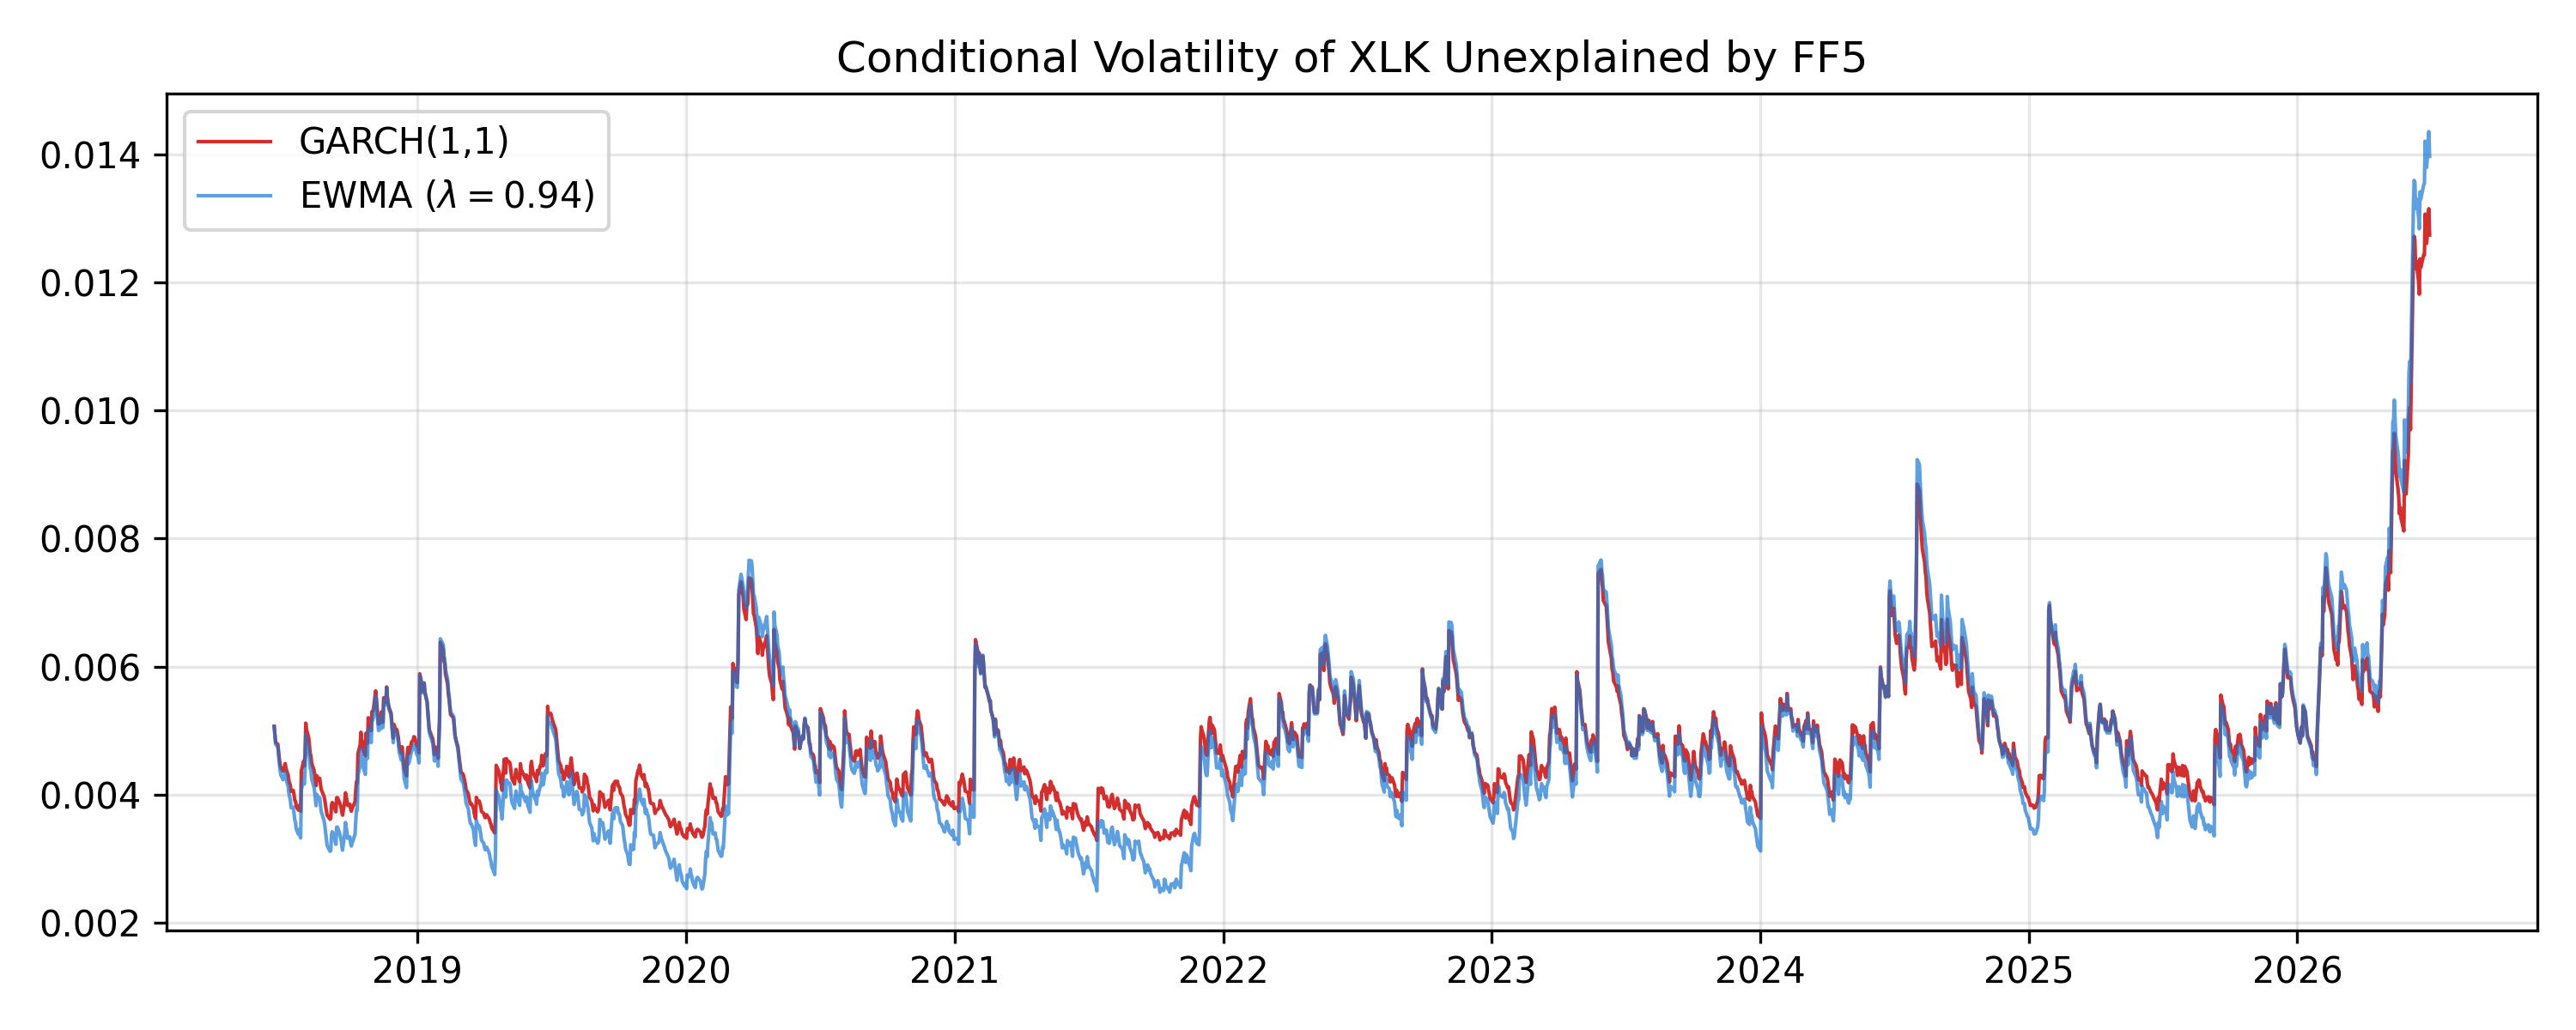
\includegraphics[width=\textwidth]{images/garch_xlk.png}
    \caption{Conditional volatility of XLK unexplained by FF5, GARCH(1,1) versus EWMA.}
    \label{fig:garch_xlk}
\end{figure}

\subsection{Sector-Momentum Baseline}

For contrast, a cross-sectional sector-momentum strategy (each month, hold the top three of eleven sector ETFs by trailing six-month return, equal weight) is benchmarked against SPY. Net of costs it returns 9.5\% versus SPY's 12.0\%, with a Sharpe of 0.53 versus 0.68 and an alpha of $-1.1\%$ ($t=-0.48$); it lowers maximum drawdown ($-16.4\%$ versus $-24.8\%$) but does not beat the benchmark on a risk-adjusted basis (Table \ref{tab:strat_metrics}). This negative result is instructive: naive cross-sectional sector momentum is hard to monetize, whereas timing a factor by its own variance, as in Section 3, is not.

\begin{table}[H]
    \centering
    \begin{tabular}{lcc}
        \toprule
        \textbf{Performance Metric} & \textbf{Momentum Rotation (Top 3)} & \textbf{SPY Benchmark} \\
        \midrule
        Annualized Return & 9.54\% & 12.03\% \\
        Annualized Volatility & 15.47\% & 15.32\% \\
        Sharpe Ratio & 0.53 & 0.68 \\
        Sortino Ratio & 0.85 & 0.96 \\
        Maximum Drawdown & $-16.35$\% & $-24.80$\% \\
        Calmar Ratio & 0.58 & 0.48 \\
        Average Turnover & 29.8\% & N/A \\
        Alpha vs SPY & $-1.11$\% ($t=-0.48$) & N/A \\
        \bottomrule
    \end{tabular}
    \caption{Sector-momentum baseline versus SPY (net of costs).}
    \label{tab:strat_metrics}
\end{table}

\section{Limitations}

\begin{itemize}[nosep]
    \item The normalization constant $c$ uses full-sample volatility for comparability; the timing signal itself is out of sample, but a strict ex-ante backtest would estimate $c$ on an expanding window.
    \item The inverse-variance weights imply leverage that can be large; the headline numbers are gross of leverage caps, and we report turnover and net-of-cost Sharpe to make the drag explicit.
    \item Realized variance over a one-month window is a simple volatility proxy; a GARCH or range-based estimator could refine the signal.
    \item The market-factor result is sample-dependent and appears to have decayed, a caution against extrapolating any single factor's timing alpha forward.
\end{itemize}

\section{Conclusion}

Volatility timing is not a free lunch across the board; it is a targeted one. On the Fama-French five factors and momentum over six decades, scaling exposure by inverse recent variance earns large, significant, cost-surviving alpha on momentum and profitability, the factors whose crashes cluster in turbulent states, and little or nothing elsewhere. The honest, factor-dependent answer is more useful than a blanket claim, and it points to where conditional risk models add value in practice.

\medskip
\noindent\textbf{Code and data:} \url{https://github.com/tanishhky/Equity-Factor-Volatility-Analysis} (all results reproducible via \texttt{src/vol\_managed\_factors.py}; this is a research and educational project, not investment advice).

\begin{thebibliography}{9}
\bibitem{moreira2017} A. Moreira and T. Muir, ``Volatility-managed portfolios,'' \textit{The Journal of Finance}, vol. 72, no. 4, pp. 1611 to 1644, 2017.
\bibitem{barroso2015} P. Barroso and P. Santa-Clara, ``Momentum has its moments,'' \textit{Journal of Financial Economics}, vol. 116, no. 1, pp. 111 to 120, 2015.
\bibitem{fama1993} E. F. Fama and K. R. French, ``Common risk factors in the returns on stocks and bonds,'' \textit{Journal of Financial Economics}, vol. 33, no. 1, pp. 3 to 56, 1993.
\bibitem{carhart1997} M. M. Carhart, ``On persistence in mutual fund performance,'' \textit{The Journal of Finance}, vol. 52, no. 1, pp. 57 to 82, 1997.
\bibitem{fama2015} E. F. Fama and K. R. French, ``A five-factor asset pricing model,'' \textit{Journal of Financial Economics}, vol. 116, no. 1, pp. 1 to 22, 2015.
\bibitem{bollerslev1986} T. Bollerslev, ``Generalized autoregressive conditional heteroskedasticity,'' \textit{Journal of Econometrics}, vol. 31, no. 3, pp. 307 to 327, 1986.
\end{thebibliography}

\end{document}
